\chapter{Evaluation}
This chapter is an evaluation of the project management and result of this project.
\section{Project Management and Schedule}
% 本项目通过学校Git进行项目管理,将项目甘特图转化为了Git中的Milestone,如图\fref{fig:milestone}所示,并且将项目分解为不同的需求和步骤列在了项目的Board中,如图fref{fig:board}所示。项目进度严格按照Miles中的时间线进行,如期完成了文档,设计,开发以及测试活动。
The project was managed through the university-owned Git. The project Gantt chart shown in \fref{fig:gannt} was converted into a Milestone in Git, as shown in figure \fref{fig:milestone}, and the project was broken down into different requirements and steps listed in the project board, as shown in figure \fref{fig:board}. The project progressed strictly according to the timeline in Milestone, and completed the documentation, design, development, and testing activities on schedule.
\begin{figure}[H]
    \centering
    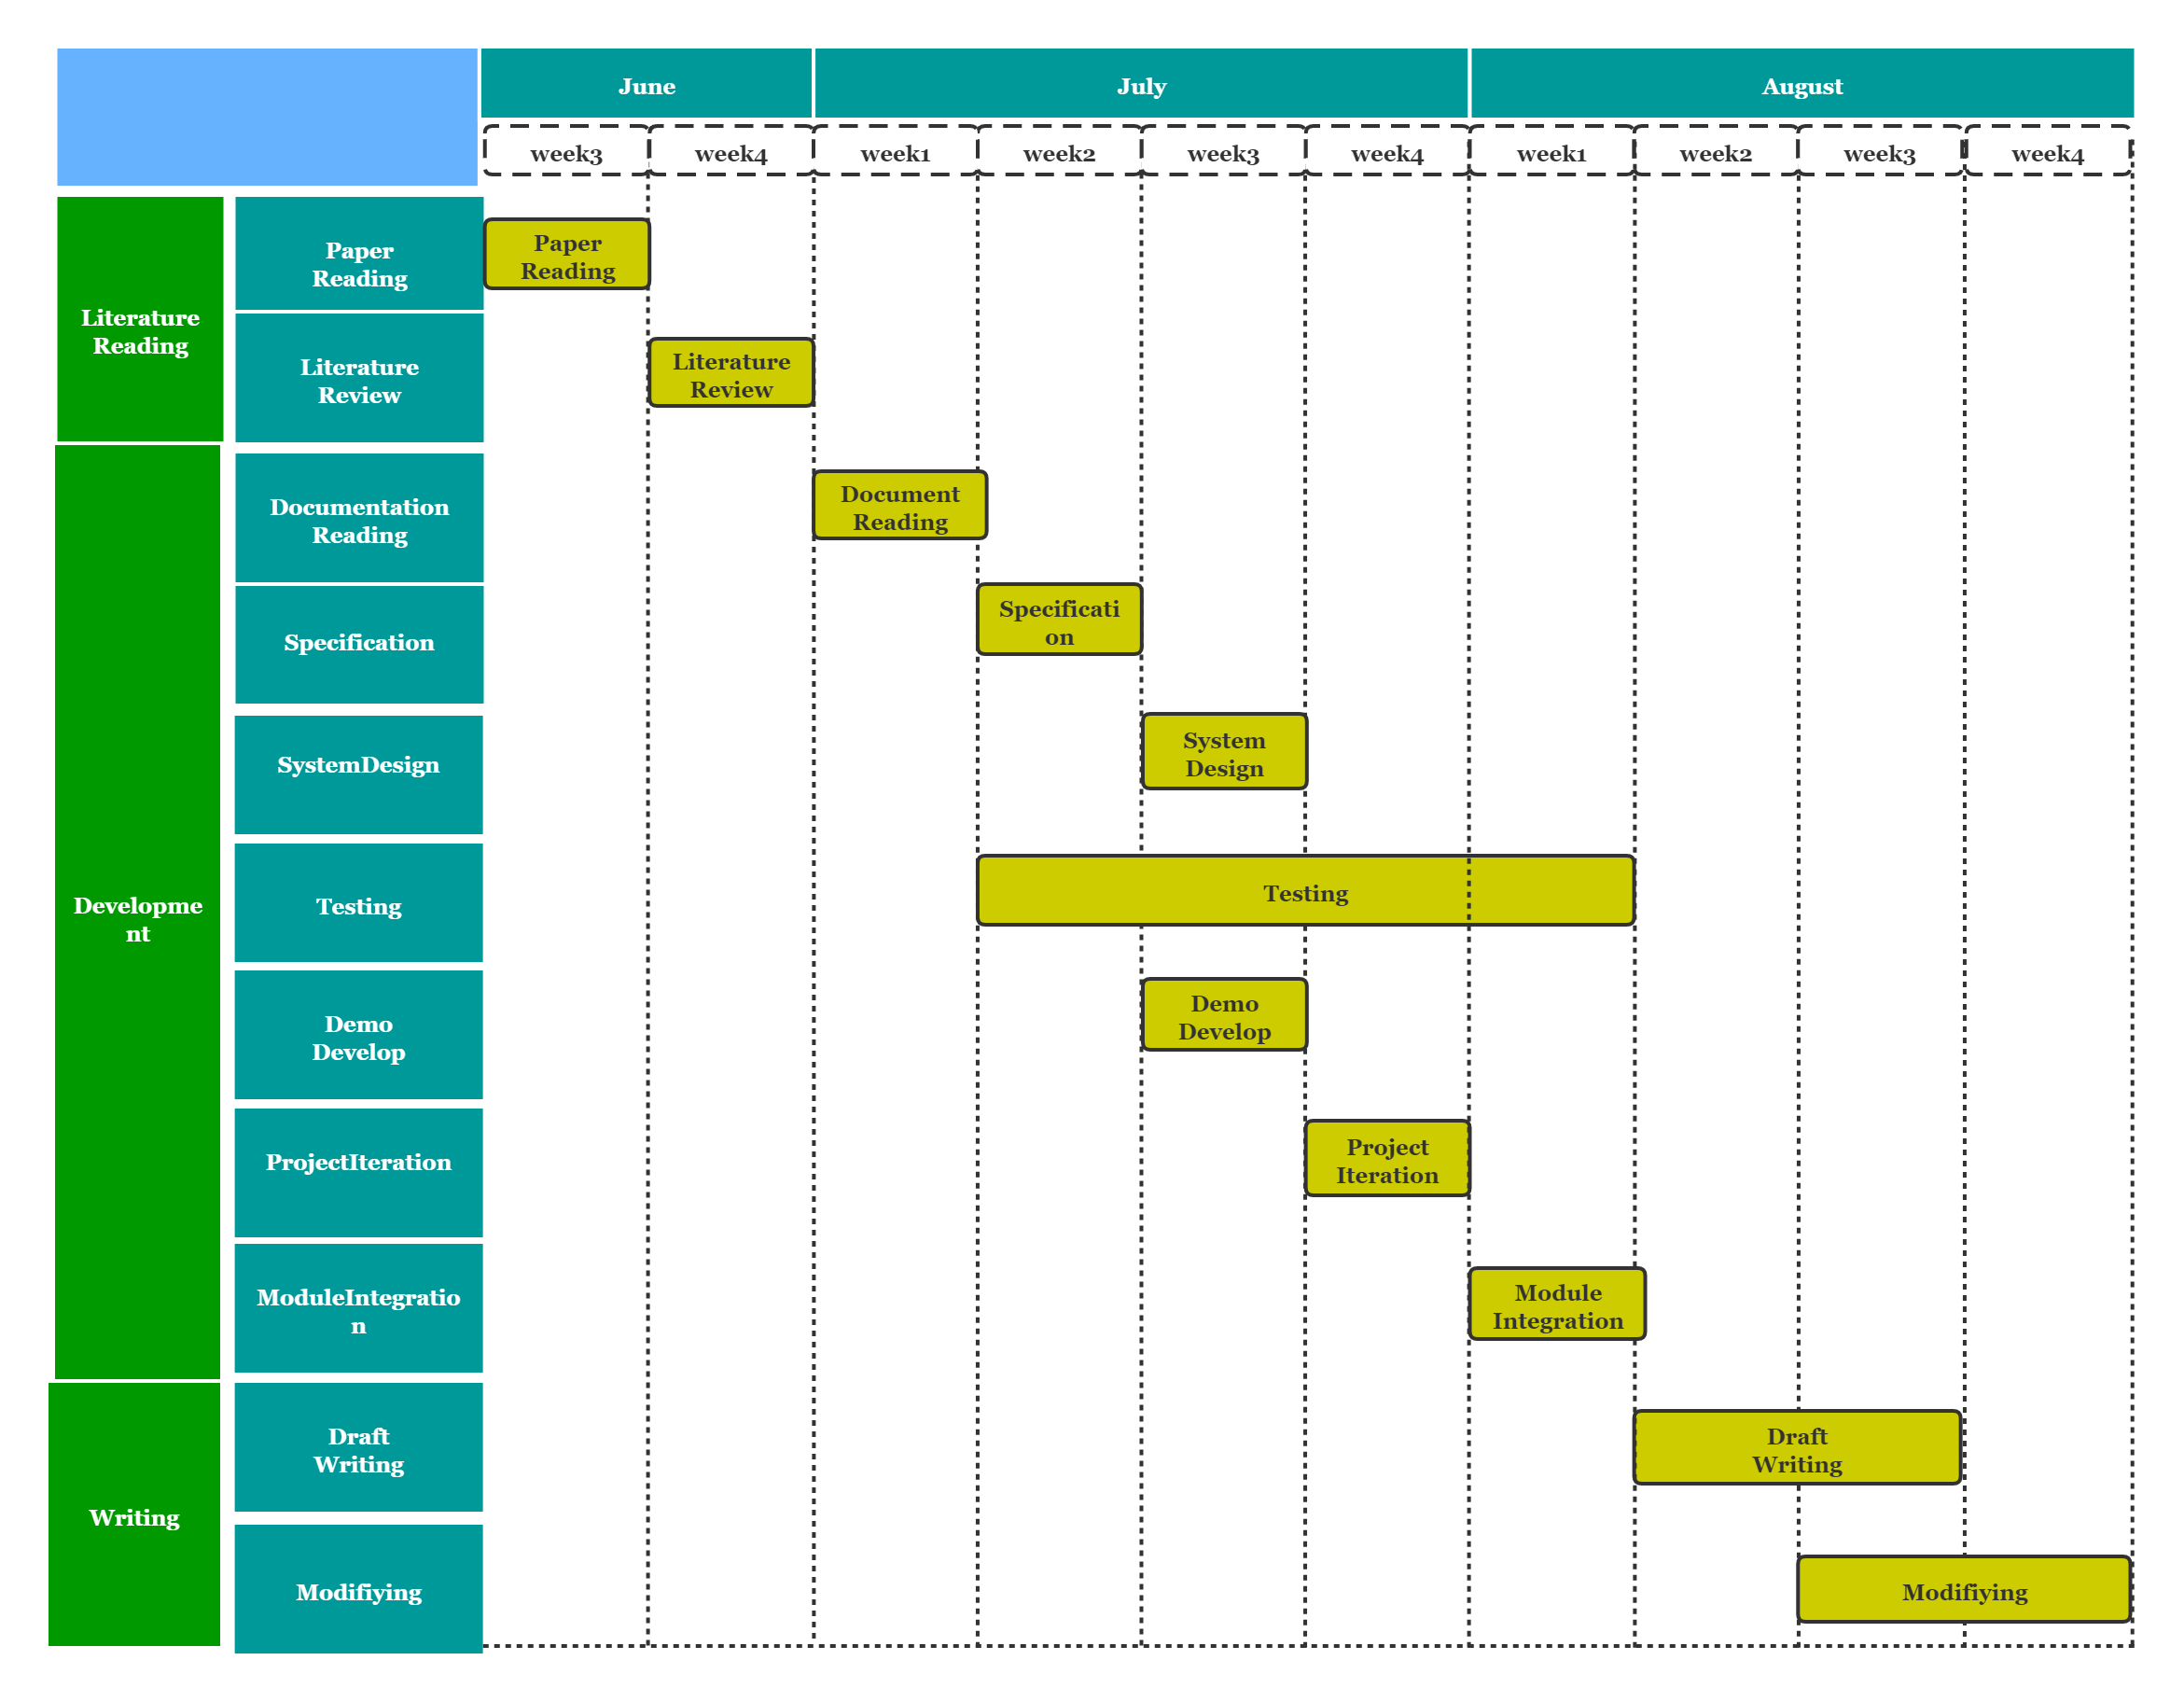
\includegraphics[width= .7 \textwidth]{img/gant.png}
    \caption{Gannt chart of the project}
    \label{fig:gannt}
\end{figure}
\begin{figure}[H]
    \centering
    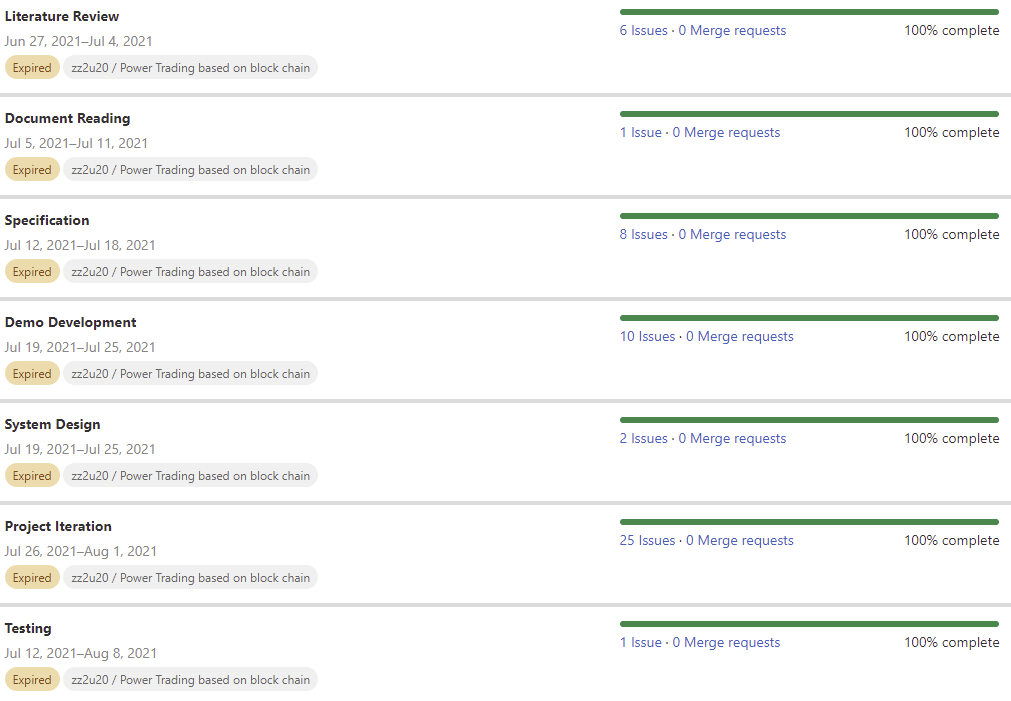
\includegraphics[width= .8 \textwidth]{img/milestone.png}
    \caption{Milestone of the project}
    \label{fig:milestone}
\end{figure}
\begin{figure}[H]
    \centering
    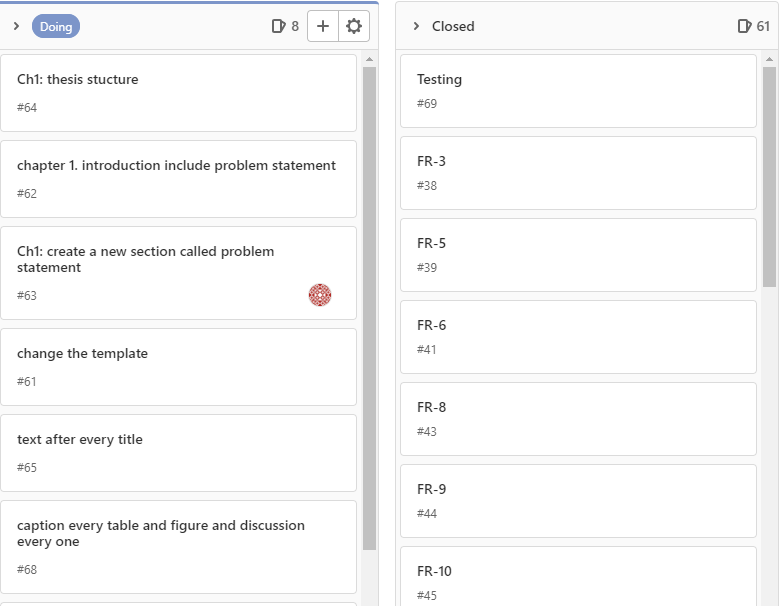
\includegraphics[width= .6 \textwidth]{img/board.png}
    \caption{Task board of the project}
    \label{fig:board}
\end{figure}

\section{Features of Project}
% 正如文献综述所说,目前市场并没有适合个人投资者进入的且能够联通清洁电力交易市场和碳排放市场的平台或者应用,因此本项目弥补了一个市场空白,根据软件实施,测试和验证章节的结果,本项目实现了一个有着界面简单,用户体验友好,交易确认速度快,稳定可靠的清洁能源交易平台。
As stated in the literature review, there is no platform or application for individual investors to enter the market that can link the clean power trading market and the carbon market, so this project fills a gap in the market. Based on the results of the software implementation, testing and validation chapter, this project achieves a clean power trading platform with features of simple interface, user-friendly experience, fast transaction confirmation, and stable and reliable.